% Generated by documents/paper/figures/make_rq_appendix.py from the rq00_task_reformulation README; do not edit.
\clearpage
\section{Task reformulation}
\label{app:rq00_task_reformulation}

\begin{rqfinding}
1. \textbf{Dropping the letters moves whole families across the gate.} At 1.7B the \texttt{rf\_} twins pass in 86 of 105 belebele, 35 of 37 Global-MMLU and 31 of 43 INCLUDE tasks (McNemar twin-only : original-only 82 : 1, 34 : 0 and 29 : 1; p $\leq$ 5.8e-08). (Figure~\ref{fig:app_rq00_task_reformulation}.)

2. \textbf{The margin gain is larger at 1.7B than at 90M.} rf $-$ original goes from +0.030 / +0.017 / +0.004 at 90M to \textbf{+0.098 / +0.058 / +0.047} at 1.7B (belebele / Global-MMLU / INCLUDE), significant at 1.7B in 56 of 59, 26 of 29 and 18 of 36 tasks. belebele and INCLUDE grow at every size, while Global-MMLU dips to +0.009 at 175M and passes its 90M value again only from 600M (+0.019).

3. \textbf{The Gemini rewrite adds more where it exists.} \texttt{rfgm\_} gains \textbf{+0.168} on belebele (59 of 59 tasks significant) and \textbf{+0.075} on INCLUDE (22 of 36) at 1.7B. \texttt{rfgm\_belebele} passes the gate in 59 of 59 tasks at every size, and \texttt{rfgm\_include\_base\_44} in 32 of 43 at 1.7B.
\end{rqfinding}

\paragraph{Question.} Do letter-format multiple-choice benchmarks leave chance at 90M--1.7B once the letters are dropped (\texttt{rf\_}) or the items are rewritten as cloze statements (\texttt{rfgm\_}), and do the reformulated twins then rank designs better?

\paragraph{Setup.} The letter-format multiple-choice benchmarks (Belebele, Global-MMLU, INCLUDE) against two reformulated twins of every task: the answer letters dropped and each option scored as a continuation (RF), and the items rewritten as cloze statements by an LLM (LLM-RF). The same above-chance gate and runs as the gate itself; original and twin are paired on the task and compared with a McNemar test.

\begin{figure}[h]
\centering
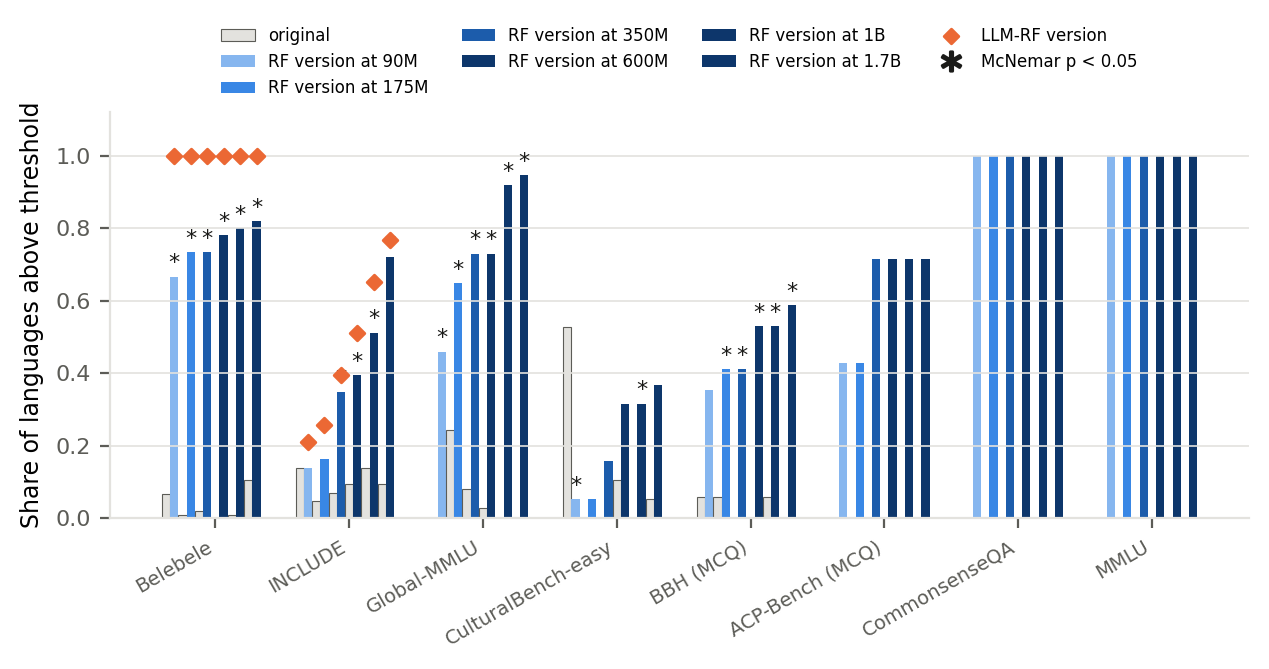
\includegraphics[width=\textwidth]{figures/app_chance_reformulation.png}
% source: src/signal-and-noise/analysis/rq00_task_reformulation/reformulations_gate_paper.png
\caption{The reformulations and the gate.}
\label{fig:app_rq00_task_reformulation}
\end{figure}
